\chapter{Operaciones cuánticas} % {{{

%Adoptando la descripción de estados cuánticos en términos de la matriz de 
%densidad $\rho$ podemos describir la dinámica de ellos como
%\begin{align*}
%	\rho '=\mathcal{E} (\rho).
%\end{align*}
%El mapeo $\mathcal{E}$ define a una operación cuántica. Esta es la 
%representación matemática de la evolución dinámica que ocurre como
%resultado de un proceso físico, $\rho$ es el estado inicial del 
%sistema y $\mathcal{E}(\rho)$ el estado final.
%
%Una manera natural de describir la dinámica de un sistema cuántico
%abierto es considerarlo que resulta de la interacción del sistema
%de interés, el sistema principal, y un entorno, que juntos forman
%un sistema cuántico cerrado. En general, el estado final 
%del sistema $\E (\rho)$ no está relacionado al estado inicial
%mediante una transformación unitaria. Vamos a asumir que
%el estado del sistema completo se encuentra en un estado
%producto, $\rho \otimes \sigma$, donde $\sigma$ es el 
%estado en el que se encuentra el entorno. Luego de la
%transformación $U$ el sistema ya no interactúa con el 
%entorno y por ello realizamos una operación de traza parcial sobre 
%el entorno para obtener el estado reducido del sistema principal:
%\begin{align}
%	\E (\rho) = \Tr _{env}\qty[U \qty(\rho \otimes \sigma)U^{\dagger}].
%	\label{eq:PTraceE(rho)}
%\end{align}
%Esta definición de operación cuántica puede tener problemas
%de generalidad dado que se hizo la suposición de que el 
%estado inicial del sistema total era un estado producto. En 
%general este no es el caso, sin embargo el formalismo de las 
%operaciones cuánticas describe también la dinámica cuántica
%de sistemas que no se encuentran inicialmente en un estado
%producto.
%
%Una definición más apropiada de las operaciones cuánticas es
%definirlo como la clase de mapeos que surgen como resultado de
%los siguientes procesos: algún sistema inicial se prepara en un
%estado cuántico desconocido $\rho$ y luego se pone en contacto
%con otros estados preparados en estados estándar, permitiendo 
%la interacción mediante alguna evolución unitaria y luego
%se desecha alguna parte del sistema total, dejando así 
%sólo al sistema final en algún estado $\rho'$. En conclusión, 
%una operación cuántica $\E$ es un mapeo de $\rho$ a $\rho'$.
%
%\section{Representación de suma de operadores}
%Las operaciones cuánticas se pueden representar de una manera
%conocida como la representación de operadores de suma. Esta
%representación es reescribir la ecuación \eqref{eq:PTraceE(rho)}
%en término de operadores que actúan sobre el sistema de Hilbert
%principal. EL resultado está motivado por el siguiente cálculo. 
%Supongamos que $\ket{e_k}$ es una base ortonormal para el
%espacio de estados del entorno y sea $\sigma = \dyad{e_0}{e_0}$
%el estado inicial del entorno. No hay perdida de generalidad si 
%asumimos que el entorno comienza en un estado producto. De 
%esta manera, la ecuación \eqref{eq:PTraceE(rho)} se convierte en
%\begin{align*}
%	\E (\rho) &= \sum _k \bra{e_k}U\qty[\rho \otimes \dyad{e_0}{e_0}]U^{\dagger}
%	\ket{e_0} \\
%						&= \sum _k E_k\rho E_k^{\dagger},
%\end{align*}
%donde $E_k\equiv \matrixel{e_k}{U}{e_k}$ es un operador que actúa
%sobre el espacio de estados del sistema principal. Los operadores
%$E_k$ se conocen como elementos de operación para la operación 
%cuántica $\E$. 
%
%\begin{align*}
%	1 &= \Tr \qty(\Erho) \\
%		&= \Tr \qty(\sum _k E_k\rho E_k^{\dagger}) \\
%		&= \Tr \qty(\sum _k E_k^{\dagger}E_k \rho),
%\end{align*}
%esto se debe cumplir para cualquier $\rho$, entonces 
%\begin{align}
%	\sum _k E_k^{\dagger}E_k = \mathbb{1}.
%\end{align}
%Esta ecuación la satisfacen las operaciones cuánticas que preservan
%la traza. No obstante, también existen operaciones cuánticas que 
%no preservan la traza, las cuales $\sum _kE_k^{\dagger}E_k\leq \mathbb{1}$,
%pero describen procesos en los que información extra sobre lo que ocurrió
%en el proceso se obtiene por medición. 
%
%La representación en operadores de suma es importante porque ofrece
%una manera intrínseca de caracterizar la dinámica del sistema principal. 
%Este formalismo describe la dinámica del sistema principal sin hacerse
%necesario considerar de manera explícita las propiedades del entorno. 
%Esto provee de implicaciones teóricas considerables. 
%
%\subsection{Enfoque axiomático}
%Ahora vamos a adoptar una ruta distinta para las operaciones cuánticas
%en la que vamos a intentar enunciar axiomas motivados físicamente que
%esperamos que cumplan las operaciones cuánticas. Esta ruta es por supuesto
%más abstracta que la anterior, pero es esta misma abstracción lo que hace
%este enfoque muy poderoso.
%
%Para proceder con este enfoque vamos a definir a las operaciones 
%cuánticas de acuerdo con un conjunto de axiomas justificados en
%bases físicas. Luego, vamos a probar que un mapeo $\E$ satisface
%estos axiomas si y sólo si tiene una representación de operadores
%de suma. De esta manera se provee del puente teórico entre 
%la formulación axiomática y la formulación motivada físicamente.
%
%Vamos definir una operación cuántica $\E$ como un mapeo del conjunto
%de los operadores de densidad del espacio de entrada $Q_1$ al 
%conjunto de los operadores de densidad del espacio de salida $Q_2$,
%con las siguientes tres propiedades axiomáticas:
%\begin{description}
%	\item[A1] \label{axiom1}
%	$\Tr \qty[\E (\rho)]$ es la probabilidad de que un proceso
%	representado por $\E$ suceda, cuando $\rho$ es el estado inicial. 
%	De esa manera, $0\leq \Tr \qty[\E (\rho)]\leq 1$ para cualquier
%	estado $\rho$.
%	\item[A2] $\E$ es un mapeo lineal convexo sobre el conjunto de las 
%	matrices de densidad. Es decir que, para un conjunto
%	de probabilidades $\{ p_i\}$,
%	\begin{align}
%		\E \qty(\sum _i p_i\rho_i) = \sum _i p_i \E \qty(\rho_i).
%		\label{eq:qtmOp-a2}
%	\end{align}
%	\item[A3] $\E$ es un mapeo completamente positivo. Es decir, si $\E$ 
%	mapea operadores de densidad del sistema $Q_1$ en operadores de
%	densidad del sistema $Q_2$, entonces $\E (A)$ debe de ser positivo
%	para cualquier operador $A$. Además, si se introduce un sistema
%	extra $R$ de dimensión arbitraria, debe ser cierto que $\qty(
%	\mathbb{1}\otimes \E)(A)$ es un operador positivo para cualquier
%	operador $A$ sobre el sistema combinado $RQ_1$, donde $\mathbb{1}$
%	denota el mapeo de la identidad sobre el sistema $R$.
%\end{description}
%
%Una operación cuántica física es aquella que satisface el 
%requisito de que las probabilidades nunca suman más de 1,
%$\Tr \qty[\E (\rho)]\leq 1$.
%
%La segunda propiedad proviene de un requisito físico sobre las
%operaciones cuánticas. Supongamos que la entrada $\rho$ de la 
%operación cuántica se obtiene aleatoriamente seleccionando un 
%estado del ensamble $\qty{ p_i,\rho_i}$ de estados cuánticos, 
%es decir que $\rho = \sum_i p_i\rho_i$. Entonces se espera que
%el estado resultante, $\E (\rho)/\Tr \qty[\E (\rho)] =
%\E (\rho)/p\qty(\E)$ corresponda a una selección aleatoria del
%ensamble $\qty{p\qty(i\vert\E), \E (\rho)/\Tr \qty[\E (\rho)]}$,
%donde $p\qty(i\vert\E)$ es la probabilidad de que el estado
%preparado fuese $\rho_i$, dado que el proceso representado por
%$\E$ ocurrió. De esa manera, se debe querir que
%\begin{align}
%	\E (\rho) = p\qty(\E)\sum _i p\qty(i\vert \E)\frac{\E (\rho)}
%	{\Tr \qty[\E (\rho)]},
%	\label{eq:e(rho)-bayes}
%\end{align}
%donde $p\qty(\E)=\Tr \qty[\E (\rho)]$ is la probabilidad de que 
%el proceso descrito por $\E$ suceda en alguna entrada de $\rho$.
%Por la regla de Bayes,
%\begin{align}
%	p\qty(i\vert \E)=p\qty(\E \vert i) \frac{p_i}{p\qty(\E)}
%	=\frac{\Tr \qty[\E (\rho)]p_i}{p\qty(\E)},
%\end{align}
%de manera que \eqref{eq:e(rho)-bayes} se reduce a \eqref{eq:qtmOp-a2}.
%
%La tercera propiedad se origina de que no sólo $\E (\rho)$ debe ser
%una matriz de densidad válida tanto cuánto $\rho$ sea válida, pero 
%además, si $\rho _{RQ}$ es la matriz de densidad de un sistema 
%de dos partes $R$ y $Q$, si $\E$ actúa sólamente sobre $Q$, 
%entonces $\E(\rho_{RQ})$ debe ser también una matriz de densidad 
%válida del sistema completo. Supongamos que introducimos un sistema 
%$R$ finito dimensional. Sea $\mathbb{1}$ el mapeo identidad sobre
%el sistema $R$. Entonces el mapeo $\mathbb{1}\otimes \E$ debe
%enviar operadores positivos hacia operadores positivos.
%
%El siguiente teorema establece la equivalencia entre este enfoque 
%axiomático y los modelos de sistema-entorno y la representación
%de operadores de suma con el que se comenzó
%la discusión de las operaciones cuánticas:
%\begin{teorema}
%	El mapeo $\E$ satisface los axiomas \textbf{A1}, \textbf{A2} y 
%	\textbf{A3} si y sólo si
%	\begin{align}
%		\E(\rho) = \sum _i E_i\rho E_i^{\dagger},
%	\end{align}
%	para algún conjunto de operadores $\qty{E_i}$ que mapean el espacio
%	de Hilbert de entrada hacia el espacio de Hilbert de salida, y
%	$\sum _kE_k^{\dagger}E_k\leq \mathbb{1}$.
%\end{teorema}

- Introducción hablando de que las operaciones cuánticas sirven 
para describir la dinámica de los sistemas abiertos y una guía al 
lector de qué se viene en este cap. Enfatizar en que el truco es 
considerar como 'nuevo sistema cerrado' al sistema extendido
\cpnote{No entiendo esa frase}
\janote{Me refiero a que un sistema que interactúa con su entorno es abierto, 
pero si consideramos al sistema total (principal+entorno) ese es cerrado.
\textbf{Ahora que lo expliqué ya no encuentro sentido para hablar de esto aquí,
mejor lo voy a quitar}}
\section{Mapeos completamente positivos}
%- Introducir la transformación de la matriz de densidad $\rho$ y hablar
%de que $\E$ transforma estados en estados.
Los estados cuánticos se transforman como \cite{nielsen_chuang_2011}
\begin{align}
\rho' = \E (\rho)
\label{eq:E(rho)},
\end{align} 
donde $\E$ es una operación cuántica. En el capítulo anterior hemos 
establecido dos ejemplos de operaciones cuánticas, la evolución unitaria 
y medición, para los cuales $\E \qty(\rho)=U\rho U^{\dagger}$ y 
$\E(\rho)=M\rho M^{\dagger}$. Una operación cuántica proporciona
una descripción discreta del cambio dinámico que un estado cuántico 
que atraviesa de un proceso físico; $\rho$ es el estado inicial y $\E (\rho)$ es el 
estado final que resulta del proceso. Una operación cuántica $\E$ es
una transformación que mapea matrices de densidad en matrices 
de densidad \cite{bengtsson_zyczkowski_2017}. ¿Será eso
suficiente para asegurar que $\E$ representa una operación física? En esta 
sección veremos que no.  Para que $\E$ sea una operación física 
debe satisface adicionalmente la condición de completa positividad. Para 
motivar la \textit{necesidad} de esta condición consideremos la operación 
que deforma la esfera de Bloch en un disco sobre el plano $XY$. Es decir,
\begin{align}
\frac{1}{2}\mqty(1+r_z&r_x-ir_y\\r_x+ir_y&1-r_z) &\longrightarrow
\frac{1}{2}\mqty(1&r_x-ir_y\\r_x+ir_y&1)
\end{align}
%\left(
%\begin{array}{cccc}
%(1+z_1)(1+z_2) & 0 & 0 & (x_1-iy_1)(x_2-iy_2) \\
%0 & 0 & 0 & 0 \\
%0 & 0 & 0 & 0 \\
%(x_1+iy_1)(x_2+iy_2) & 0 & 0 &(1-z_1)(1-z_2)\\
%\end{array}
%\right) &\longrightarrow
%\left(
%\begin{array}{cccc}
%1+z_2 & 0 & 0 & (x_1-iy_1)(x_2-iy_2) \\
%0 & 0 & 0 & 0 \\
%0 & 0 & 0 & 0 \\
%(x_1+iy_1)(x_2+iy_2) & 0 & 0 &1-z_2\\
%\end{array}
%\right)\\
%1-\sqrt{\text{x}_1^2 \text{x2}^2+\text{x1}^2 
%    \text{y2}^2+\text{x2}^2 \text{y1}^2+\text{y1}^2 \text{y2}^2+\text{z2}^2}
%\end{align}

\begin{figure}[H]
\centering
\begin{minipage}{.4\textwidth}
\centering
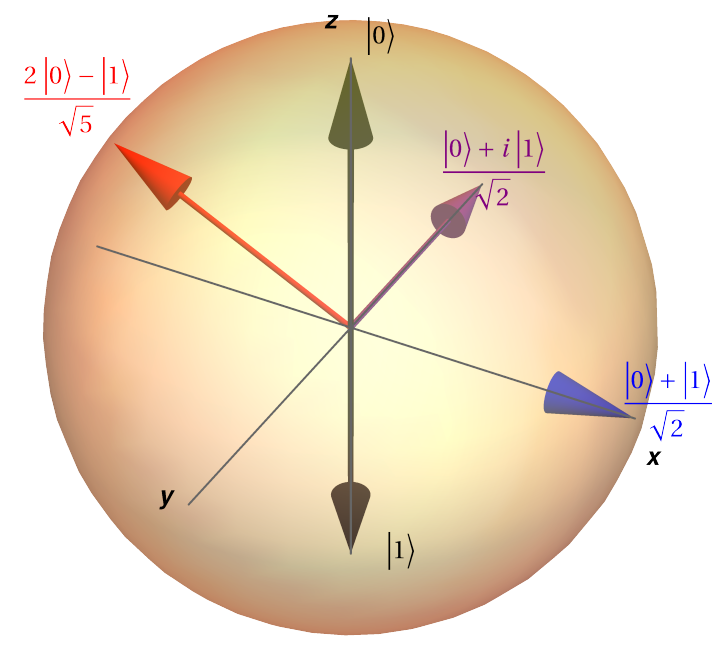
\includegraphics[width=5cm]
{img-congreso/bloch.png}
\end{minipage}
$\stackrel{\E_{z}\otimes\1 \vspace{1cm}}{\longmapsto}$
\begin{minipage}{0.4\textwidth}
\centering
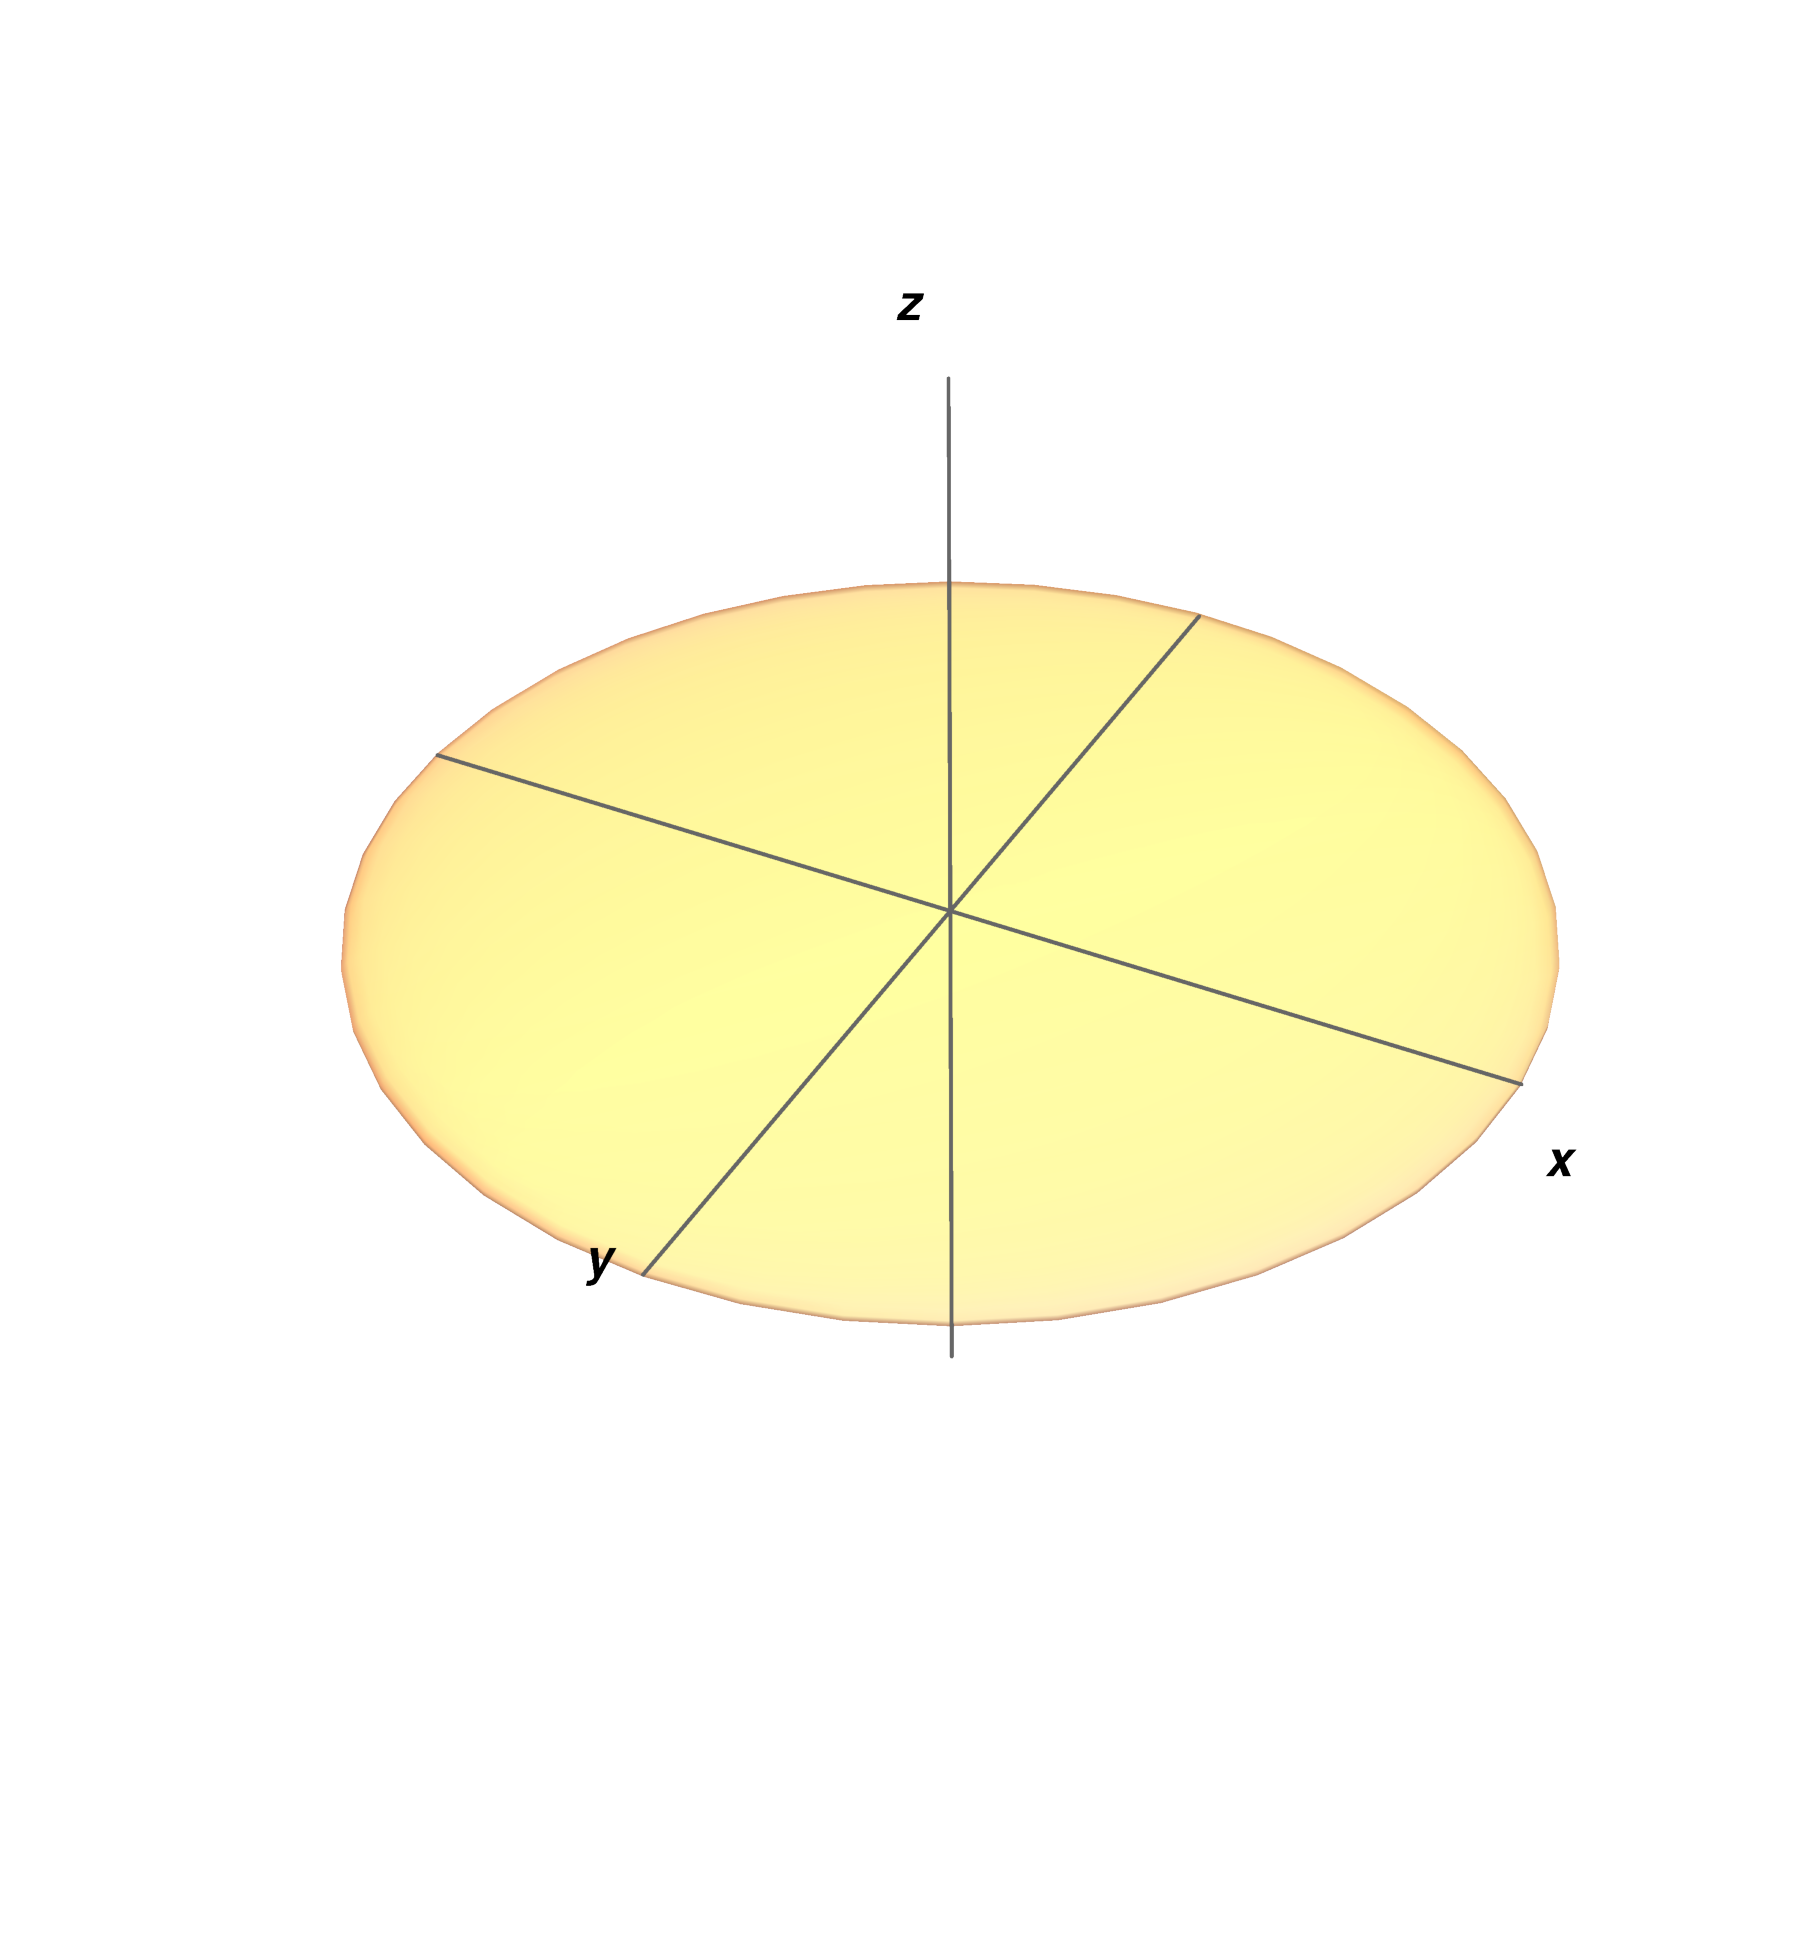
\includegraphics[width=6cm]
{img-congreso/DiskXY}
\end{minipage}
\caption{Deformación de la esfera de Bloch a un disco sobre el plano $XY$.}
\end{figure}

\begin{align}
\rho&=\sum _{i,j}r_{ij}\sigma_i\otimes\sigma_j
\end{align}

$r_{00}=1/4$, $r_{03}=r_{30}=0$ y $r_{33}=1/4$
\begin{align}
%\rho^{\phi}&=
\mqty( 
\frac{1}{2} & 0 & 0 & \frac{1}{2} \\
0 & 0 & 0 & 0 \\
0 & 0 & 0 & 0 \\
\frac{1}{2} & 0 & 0 & \frac{1}{2} \\
)
%\E\otimes\1\qty(\rho^{\phi})&=
\stackrel{\E_{z}\otimes\1}{\longrightarrow}
\mqty( 
\frac{1}{4} & 0 & 0 & \frac{1}{2} \\
0 & \frac{1}{4} & 0 & 0 \\
0 & 0 & \frac{1}{4} & 0 \\
\frac{1}{2} & 0 & 0 & \frac{1}{4} \\
).
\end{align}
Uno de los autovalores de $\E\otimes\1\qty(\rho^{\phi})$ es $-1/4$, por
lo cual no es una matriz de densidad. Lo que acabamos de mostrar es que
el mapeo que deforma la esfera de Bloch a un disco sobre el plano $XY$ 
cuando actúa sobre el estado máximamente entrelazado de un sistema 
de 2 qubits da como resultado un estado que no es físico. Por consiguiente, 
este ejemplo hace evidente que una operación cuántica represente
la evolución física de los estados cuánticos no es suficiente que sea
un mapeo afín de matrices de densidad, sino también se requiere 
que la operación en un espacio extendido siga siendo un mapeo afín. 
Esta condición se conoce como completa positividad y discutiremos
a continuación la definición de ella.   

- Motivación de la CP. Ejemplo del mapeo que deforma la esfera de Bloch
en un disco: presentar que el mapeo extendido para 2 qubits
aplicado al estado máximamente entrelazado resulta en una matriz 
no positiva (algo que no es estado).

%- Definición de CP del Geometry of Quantum States.
Una operación $\E$ se dice que es completamente positiva
si y sólo si, para cualquier extensión dimensional arbitraria $K$ tal que 
$\hi_N \rightarrow \hi_N \otimes \hi_K$,
el operador $\E\otimes\1$ es positivo semidefinido 
\cite{bengtsson_zyczkowski_2017}.

- Concluir con que las operaciones que estudiamos deben ser CPTP.


\section{Superoperadores}
\janote{Propongo agregar esta sección por la línea que quiero seguir 
durante todo el capítulo. Además que si menciono la representación en 
suma de operadores, por qué no la de superoperadores?  es la que he 
usado para la parte numérica}

%- Empezar hablando del reshape a $\rho$ (pasarlo de matriz a vector columna)
Consideremos una matriz rectangular $A$ de dimensión $M\times N$.
La matriz puede ser reordenada colocando sus elementos de matriz en 
orden lexicográfico en un vector $\vec{a}$ con $MN$ entradas, es decir
\begin{align}
a_k=A_{ij}, 
\end{align}
donde $k=\qty(i-1)N+j$, con $i=,1,\ldots,M$ y $j=1,\ldots,N$.

La transformación de \textit{reshuffle} de una matriz consiste 
en reordenar cada fila de la matriz en submatrices y colocarlas en 
orden lexicográfico bloque por bloque. Veamos un ejemplo a continuación
\begin{align}
\mqty(
A_{00}&A_{01}&A_{02}&A_{03}\\
A_{10}&A_{11}&A_{12}&A_{13}\\
A_{20}&A_{21}&A_{22}&A_{23}\\
A_{30}&A_{31}&A_{32}&A_{33})
\stackrel{R}{\longrightarrow}
\mqty(
A_{00}&A_{01}&A_{10}&A_{11}\\
A_{02}&A_{03}&A_{12}&A_{13}\\
A_{20}&A_{21}&A_{30}&A_{31}\\
A_{22}&A_{23}&A_{32}&A_{33}).
\end{align}

- Hablar de los mapeos que actúan sobre $\rho$ como un vector columna 

- Hablar de la matriz de Choi y enunciar el teorema de Choi: si la matriz
 de Choi es positiva semidefinida entonces la operación cuántica es CP
 
- Concluir con un ejemplo de un canal nuestro sobre 1 qubit

\section{Representación de suma de operadores}
- Enunciar la representación en operadores de suma partiendo de un 
estado que se acopla con algún entorno
y llegar a las condiciones para ser CPTP y empezar a conectarlo
con la sección anterior. \cpnote{No sabes si hay alguna motivacion que no sea
con el entorno? Realmente no lo usamos y se me hace meter una complicación adicional}
\janote{Podría utilizar el segundo item de este cap. como motivación. Creo
que esto sí lo usamos. David revisó unas cosas así (o mencionó que quería
hacerlo)}

- Invocar el ejemplo del canal de la sección anterior, pero en su 
representación de operadores de suma. Aquí quiero hacer la conexión 
entre esta y la sección anterior mostrando que los operadores 
de Kraus son los autovectores de la matriz de Choi. 

- Comparar la representacion de suma de operadores y superoperadores


\section{Canales cuánticos de 1 qubit}
- Hablar de que se gana intuición pensando en la acción de un canal de 1
qubit como la manera en que deforma la esfera de Bloch

- Ejemplos: phase-flip channel, depolarizing y amplitude damping 

- De los ejemplos hablar sobre canales unitales? Breve. (es que nuestros
canales son unitales)

% }}}

